% !TeX program = xelatex
%
% Лекция «Текст как данные»: пять блоков, которые курс добавляет для
% направления «Цифровая лингвистика и локализация». Заменяет
% МЛГ_Текст_как_данные.pptx: те же пять блоков, но числа сверены с тем, что
% печатают ноутбуки лабораторных, и у каждого блока есть свой playground.
% По плану правки блоки читаются в разные недели (Методические/План_правки_лекций.md),
% поэтому каждый начинается с отдельного титульного слайда.
%
% Сборка:  xelatex mlg_text_as_data.tex   (дважды)
% Оформление и макросы — в mlg_preamble.tex, общем для всех лекций курса.
% Все числа посчитаны на учебном корпусе курса и закреплены тестами
% репозитория gd_learn; придуманных чисел на слайдах нет.
%
\documentclass[aspectratio=169,12pt]{beamer}

% Общая преамбула лекций курса. Подключается после \documentclass:
%
%     \documentclass[aspectratio=169,12pt]{beamer}
%     % Общая преамбула лекций курса. Подключается после \documentclass:
%
%     \documentclass[aspectratio=169,12pt]{beamer}
%     % Общая преамбула лекций курса. Подключается после \documentclass:
%
%     \documentclass[aspectratio=169,12pt]{beamer}
%     \input{mlg_preamble}
%
% Здесь только оформление и макросы — ни \title, ни текста слайдов, чтобы
% пять презентаций курса выглядели одинаково и правились в одном месте.
%
\usepackage{fontspec}
\usepackage{polyglossia}
\setmainlanguage{russian}
\setotherlanguage{english}
\setmainfont{Calibri}
\setsansfont{Calibri}
\setmonofont{Consolas}[Scale=0.92]

\usepackage{graphicx}
\usepackage{booktabs}
\usepackage{array}

% ---------------------------------------------------------------- оформление
\definecolor{ink}{HTML}{1B2433}
\definecolor{navy}{HTML}{2B4C6F}
\definecolor{brick}{HTML}{B03A2B}
\definecolor{moss}{HTML}{3E7D5A}
\definecolor{plum}{HTML}{6B5B95}
\definecolor{ash}{HTML}{8B9299}
\definecolor{paper}{HTML}{ECEFF3}

\usetheme{default}
\usecolortheme{default}
\setbeamercolor{structure}{fg=navy}
\setbeamercolor{frametitle}{fg=navy}
\setbeamercolor{normal text}{fg=ink}
\setbeamercolor{itemize item}{fg=navy}
\setbeamercolor{itemize subitem}{fg=ash}
\setbeamerfont{frametitle}{size=\Large,series=\bfseries}
\setbeamerfont{framesubtitle}{size=\small,series=\mdseries}
\setbeamercolor{framesubtitle}{fg=ash}
\setbeamertemplate{navigation symbols}{}
\setbeamertemplate{itemize item}{\raisebox{0.15ex}{\tiny$\bullet$}}
\setbeamertemplate{itemize subitem}{\raisebox{0.15ex}{\tiny--}}
\setbeamersize{text margin left=1.1cm, text margin right=1.1cm}

\setbeamertemplate{footline}{%
  \hbox{\begin{beamercolorbox}[wd=\paperwidth,ht=2.6ex,dp=1.4ex,leftskip=1.1cm,%
        rightskip=1.1cm]{}%
    {\color{ash}\scriptsize Основы машинного обучения \quad·\quad
     Цифровая лингвистика и локализация}\hfill
    {\color{ash}\scriptsize\insertframenumber}%
  \end{beamercolorbox}}}

% Врезка: связь слайда с лабораторной или с работой переводчика.
% Ширина считается точно: colorbox добавляет \fboxsep с каждой стороны,
% поэтому parbox должен быть на 2\fboxsep уже текстового поля — иначе
% на каждом слайде вылезает overfull hbox.
\newcommand{\врезка}[1]{%
  \par\vspace{0.5ex}\noindent
  \colorbox{paper}{%
    \parbox{\dimexpr\textwidth-2\fboxsep\relax}{%
      \vspace{0.7ex}\small #1\vspace{0.7ex}}}\par}

% Колонка таблицы заданной доли ширины, без растягивания пробелов.
% Объявлять её нужно здесь: внутри frame beamer пересканирует тело кадра,
% и #1 в определении вызывает «Illegal parameter number».
\newcolumntype{Л}[1]{>{\raggedright\arraybackslash}p{#1\textwidth}}

% Ссылка на интерактивную страницу к слайду. Playground'ы считают те же
% числа на том же корпусе, что и лабораторные, поэтому на них можно
% ссылаться прямо с лекции, не оговаривая расхождений.
\hypersetup{colorlinks=true,urlcolor=moss,linkcolor=moss}
\newcommand{\playground}[3]{%
  \par\vspace{0.4ex}%
  {\footnotesize\color{ash}$\rightarrow$~\href{#1}{\bfseries #2} — #3\par}}

\newcommand{\кейс}[1]{{\color{brick}\small\textbf{#1}}}
\newcommand{\числ}[1]{{\color{navy}\bfseries #1}}

%
% Здесь только оформление и макросы — ни \title, ни текста слайдов, чтобы
% пять презентаций курса выглядели одинаково и правились в одном месте.
%
\usepackage{fontspec}
\usepackage{polyglossia}
\setmainlanguage{russian}
\setotherlanguage{english}
\setmainfont{Calibri}
\setsansfont{Calibri}
\setmonofont{Consolas}[Scale=0.92]

\usepackage{graphicx}
\usepackage{booktabs}
\usepackage{array}

% ---------------------------------------------------------------- оформление
\definecolor{ink}{HTML}{1B2433}
\definecolor{navy}{HTML}{2B4C6F}
\definecolor{brick}{HTML}{B03A2B}
\definecolor{moss}{HTML}{3E7D5A}
\definecolor{plum}{HTML}{6B5B95}
\definecolor{ash}{HTML}{8B9299}
\definecolor{paper}{HTML}{ECEFF3}

\usetheme{default}
\usecolortheme{default}
\setbeamercolor{structure}{fg=navy}
\setbeamercolor{frametitle}{fg=navy}
\setbeamercolor{normal text}{fg=ink}
\setbeamercolor{itemize item}{fg=navy}
\setbeamercolor{itemize subitem}{fg=ash}
\setbeamerfont{frametitle}{size=\Large,series=\bfseries}
\setbeamerfont{framesubtitle}{size=\small,series=\mdseries}
\setbeamercolor{framesubtitle}{fg=ash}
\setbeamertemplate{navigation symbols}{}
\setbeamertemplate{itemize item}{\raisebox{0.15ex}{\tiny$\bullet$}}
\setbeamertemplate{itemize subitem}{\raisebox{0.15ex}{\tiny--}}
\setbeamersize{text margin left=1.1cm, text margin right=1.1cm}

\setbeamertemplate{footline}{%
  \hbox{\begin{beamercolorbox}[wd=\paperwidth,ht=2.6ex,dp=1.4ex,leftskip=1.1cm,%
        rightskip=1.1cm]{}%
    {\color{ash}\scriptsize Основы машинного обучения \quad·\quad
     Цифровая лингвистика и локализация}\hfill
    {\color{ash}\scriptsize\insertframenumber}%
  \end{beamercolorbox}}}

% Врезка: связь слайда с лабораторной или с работой переводчика.
% Ширина считается точно: colorbox добавляет \fboxsep с каждой стороны,
% поэтому parbox должен быть на 2\fboxsep уже текстового поля — иначе
% на каждом слайде вылезает overfull hbox.
\newcommand{\врезка}[1]{%
  \par\vspace{0.5ex}\noindent
  \colorbox{paper}{%
    \parbox{\dimexpr\textwidth-2\fboxsep\relax}{%
      \vspace{0.7ex}\small #1\vspace{0.7ex}}}\par}

% Колонка таблицы заданной доли ширины, без растягивания пробелов.
% Объявлять её нужно здесь: внутри frame beamer пересканирует тело кадра,
% и #1 в определении вызывает «Illegal parameter number».
\newcolumntype{Л}[1]{>{\raggedright\arraybackslash}p{#1\textwidth}}

% Ссылка на интерактивную страницу к слайду. Playground'ы считают те же
% числа на том же корпусе, что и лабораторные, поэтому на них можно
% ссылаться прямо с лекции, не оговаривая расхождений.
\hypersetup{colorlinks=true,urlcolor=moss,linkcolor=moss}
\newcommand{\playground}[3]{%
  \par\vspace{0.4ex}%
  {\footnotesize\color{ash}$\rightarrow$~\href{#1}{\bfseries #2} — #3\par}}

\newcommand{\кейс}[1]{{\color{brick}\small\textbf{#1}}}
\newcommand{\числ}[1]{{\color{navy}\bfseries #1}}

%
% Здесь только оформление и макросы — ни \title, ни текста слайдов, чтобы
% пять презентаций курса выглядели одинаково и правились в одном месте.
%
\usepackage{fontspec}
\usepackage{polyglossia}
\setmainlanguage{russian}
\setotherlanguage{english}
\setmainfont{Calibri}
\setsansfont{Calibri}
\setmonofont{Consolas}[Scale=0.92]

\usepackage{graphicx}
\usepackage{booktabs}
\usepackage{array}

% ---------------------------------------------------------------- оформление
\definecolor{ink}{HTML}{1B2433}
\definecolor{navy}{HTML}{2B4C6F}
\definecolor{brick}{HTML}{B03A2B}
\definecolor{moss}{HTML}{3E7D5A}
\definecolor{plum}{HTML}{6B5B95}
\definecolor{ash}{HTML}{8B9299}
\definecolor{paper}{HTML}{ECEFF3}

\usetheme{default}
\usecolortheme{default}
\setbeamercolor{structure}{fg=navy}
\setbeamercolor{frametitle}{fg=navy}
\setbeamercolor{normal text}{fg=ink}
\setbeamercolor{itemize item}{fg=navy}
\setbeamercolor{itemize subitem}{fg=ash}
\setbeamerfont{frametitle}{size=\Large,series=\bfseries}
\setbeamerfont{framesubtitle}{size=\small,series=\mdseries}
\setbeamercolor{framesubtitle}{fg=ash}
\setbeamertemplate{navigation symbols}{}
\setbeamertemplate{itemize item}{\raisebox{0.15ex}{\tiny$\bullet$}}
\setbeamertemplate{itemize subitem}{\raisebox{0.15ex}{\tiny--}}
\setbeamersize{text margin left=1.1cm, text margin right=1.1cm}

\setbeamertemplate{footline}{%
  \hbox{\begin{beamercolorbox}[wd=\paperwidth,ht=2.6ex,dp=1.4ex,leftskip=1.1cm,%
        rightskip=1.1cm]{}%
    {\color{ash}\scriptsize Основы машинного обучения \quad·\quad
     Цифровая лингвистика и локализация}\hfill
    {\color{ash}\scriptsize\insertframenumber}%
  \end{beamercolorbox}}}

% Врезка: связь слайда с лабораторной или с работой переводчика.
% Ширина считается точно: colorbox добавляет \fboxsep с каждой стороны,
% поэтому parbox должен быть на 2\fboxsep уже текстового поля — иначе
% на каждом слайде вылезает overfull hbox.
\newcommand{\врезка}[1]{%
  \par\vspace{0.5ex}\noindent
  \colorbox{paper}{%
    \parbox{\dimexpr\textwidth-2\fboxsep\relax}{%
      \vspace{0.7ex}\small #1\vspace{0.7ex}}}\par}

% Колонка таблицы заданной доли ширины, без растягивания пробелов.
% Объявлять её нужно здесь: внутри frame beamer пересканирует тело кадра,
% и #1 в определении вызывает «Illegal parameter number».
\newcolumntype{Л}[1]{>{\raggedright\arraybackslash}p{#1\textwidth}}

% Ссылка на интерактивную страницу к слайду. Playground'ы считают те же
% числа на том же корпусе, что и лабораторные, поэтому на них можно
% ссылаться прямо с лекции, не оговаривая расхождений.
\hypersetup{colorlinks=true,urlcolor=moss,linkcolor=moss}
\newcommand{\playground}[3]{%
  \par\vspace{0.4ex}%
  {\footnotesize\color{ash}$\rightarrow$~\href{#1}{\bfseries #2} — #3\par}}

\newcommand{\кейс}[1]{{\color{brick}\small\textbf{#1}}}
\newcommand{\числ}[1]{{\color{navy}\bfseries #1}}


\usepackage{tikz}
\usepackage{pgfplots}
\pgfplotsset{compat=1.18}

\title{Текст как данные}
\subtitle{Пять блоков к курсу «Основы машинного обучения»}
\date{}
\author{}

% Титульный слайд блока: номер, название, одна фраза о том, зачем он.
\newcommand{\блок}[3]{%
  \vspace{1.4cm}
  {\color{brick}\small\bfseries БЛОК #1\par}
  \vspace{0.6cm}
  {\color{navy}\fontsize{28}{32}\selectfont\bfseries #2\par}
  \vspace{0.6cm}
  {\color{ink}\large #3\par}}

\begin{document}

% =====================================================================
\begin{frame}[plain]
  \vspace{1.2cm}
  {\color{brick}\small\bfseries ОСНОВЫ МАШИННОГО ОБУЧЕНИЯ · ДОПОЛНИТЕЛЬНЫЕ БЛОКИ}

  \vspace{0.7cm}
  {\color{navy}\fontsize{30}{34}\selectfont\bfseries Текст как данные\par}

  \vspace{0.5cm}
  {\color{ink}\large Как язык попадает в машинное обучение и что с ним
  там происходит\par}

  \vspace{1.0cm}
  {\color{ash} Магистратура «Цифровая лингвистика и локализация». Все числа
   на слайдах — из лабораторных работ курса, на том же корпусе из 160
   сегментов локализации.\par}
\end{frame}

% =====================================================================
\begin{frame}{Пять блоков и где их потрогать руками}
  Основной курс объясняет машинное обучение на числах. Эти блоки — о том,
  как в эту схему попадает текст. Каждый привязан к лабораторной и к
  странице, где то же самое можно покрутить руками.

  \vspace{0.7em}
  {\small
  \begin{tabular}{@{}l Л{0.36} l l@{}}
    \toprule
    блок & о чём & работа & playground \\
    \midrule
    1 & текст как данные: токены, словоформы, признаки & Л.р. № 1 & векторизация \\
    2 & математический минимум: вектор, косинус, градиент & Л.р. № 2 & память переводов \\
    3 & языковые модели & Л.р. № 4 & языковая модель \\
    4 & метрики для текста & Л.р. № 3 & метрики перевода \\
    5 & данные и разметка & Л.р. № 1 и № 3 & данные и разметка \\
    \bottomrule
  \end{tabular}}

  \vspace{0.8em}
  {\footnotesize\color{ash} Все playground'ы — на
  \href{https://konkin-nikita.ru/gd_learn/}{konkin-nikita.ru/gd\_learn}:
  они считают те же числа на том же корпусе, что и ноутбуки.}
\end{frame}

% =====================================================================
% БЛОК 1
% =====================================================================
\begin{frame}[plain]
  \блок{1}{Текст как данные}{Модель видит числа. Всё, что вы знаете о
  языке, попадает в неё ровно одним способом — через то, как вы превратили
  текст в числа.}
\end{frame}

% =====================================================================
\begin{frame}{Модель не читает текст}
  \centering
  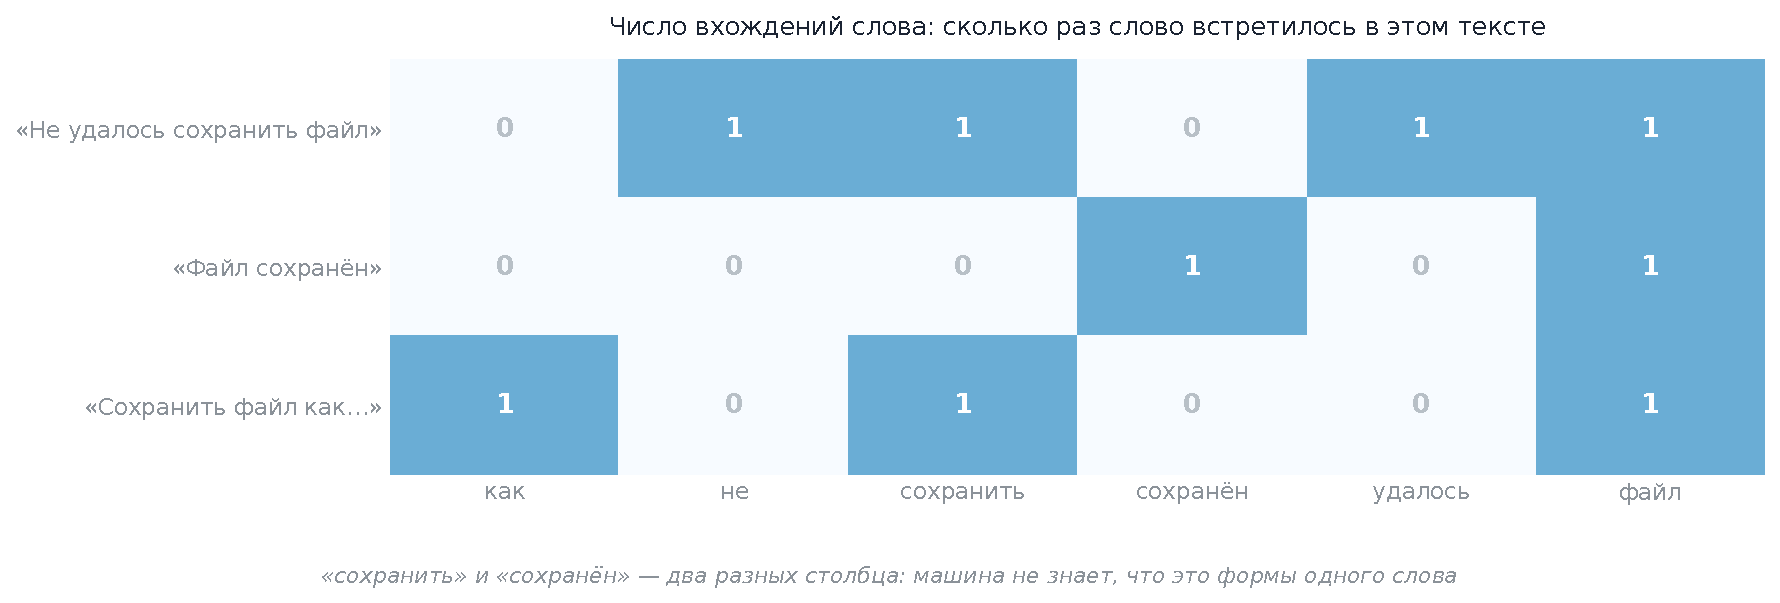
\includegraphics[width=0.82\textwidth]{fig/bagofwords.pdf}\par
  \raggedright
  \vspace{0.4em}
  {\small Любой алгоритм принимает таблицу: строка — объект, столбец —
  признак. Между текстом и моделью всегда стоит шаг векторизации, и
  проектирует его человек: выбор единицы, нормализация, отбор признаков —
  всё это решения о языке.}

  \врезка{\textbf{Л.р. № 1, раздел 8.} Один и тот же наивный Байес на одном
  и том же корпусе даёт от \числ{0{,}381} до \числ{0{,}631}. Меняется только
  способ превратить текст в признаки.}
\end{frame}

% =====================================================================
\begin{frame}{Шаг первый: токенизация}
  Разбить текст на единицы. Кажется тривиальным — до первого реального файла.

  \vspace{0.5em}
  \begin{columns}[T,onlytextwidth]
    \column{0.50\textwidth}
      {\small
      \кейс{Пунктуация:} «серверу.» и «серверу» — одна единица или две?\par
      \vspace{0.3em}
      \кейс{Дефисы:} «из-за», «кто-нибудь», «интернет-магазин».\par
      \vspace{0.3em}
      \кейс{Плейсхолдеры:} \texttt{\{name\}}, \texttt{\%s},
      \texttt{<b>} — их нельзя ни резать, ни переводить.\par
      \vspace{0.3em}
      \кейс{Числа и единицы:} «25 МБ», «02:00», «TLS 1.3».\par
      \vspace{0.3em}
      \кейс{Буква ё:} «все» и «всё» — разные слова.}
    \column{0.44\textwidth}
      \врезка{\textbf{Л.р. № 1, раздел 4.} Словарь корпуса начинается с
      \texttt{00}, \texttt{02}, \texttt{25}, \texttt{429}, \texttt{api},
      \texttt{csv}, \texttt{https}, \texttt{minutes}, \texttt{name}.
      Токенизатор по умолчанию разрезал время и превратил плейсхолдеры
      \texttt{\{minutes\}} и \texttt{\{name\}} в английские слова.}
  \end{columns}

  \vspace{0.6em}
  {\small Готовые токенизаторы: \texttt{razdel}, \texttt{nltk},
  \texttt{spaCy}. Регулярное выражение годится для учебной задачи и
  ломается на реальной.}
\end{frame}

% =====================================================================
\begin{frame}{Шаг второй: нормализация словоформ}
  \begin{columns}[T,onlytextwidth]
    \column{0.47\textwidth}
      {\color{moss}\bfseries Стемминг}\\[0.3em]
      {\small Усечение до основы по правилам. Быстро, грубо, без словаря;
      основа не обязана быть словом.\par
      \vspace{0.4em}
      \texttt{сохранены}, \texttt{сохранить} $\rightarrow$ \texttt{сохран}\par
      \texttt{изменения} $\rightarrow$ \texttt{изменен}\par
      \vspace{0.3em}
      {\color{ash}— вывод раздела 8 Л.р. № 1}}
    \column{0.47\textwidth}
      {\color{navy}\bfseries Лемматизация}\\[0.3em]
      {\small Приведение к словарной форме. Нужны словарь и снятие
      омонимии: «стали» — это «стать» или «сталь»?\par
      \vspace{0.4em}
      Для русского: \texttt{pymorphy3}, \texttt{spaCy}, \texttt{Natasha}.}
  \end{columns}

  \vspace{0.7em}
  {\small Для английского разница невелика. Для русского принципиальна:
  одна лексема даёт десятки словоформ, и без нормализации модель считает
  их не связанными между собой признаками.}

  \врезка{\textbf{Л.р. № 1:} стемминг поднимает наивный Байес с 0,444 до
  0,538 — но разброс между долями доходит до 0,135. Одна таблица этого
  не доказывает; доказывают сегменты, которые он исправил.}
\end{frame}

% =====================================================================
\begin{frame}{Шаг третий: мешок слов и TF-IDF}
  \begin{columns}[T,onlytextwidth]
    \column{0.47\textwidth}
      {\color{navy}\bfseries Мешок слов}\\[0.3em]
      {\small Словарь корпуса и число вхождений каждого слова. Порядок
      теряется полностью: «не удалось подключиться» и «удалось не
      подключиться» — один и тот же вектор.}
    \column{0.47\textwidth}
      {\color{navy}\bfseries TF-IDF}\\[0.3em]
      {\small Вес слова — произведение двух множителей: как часто оно в
      этом тексте (TF) и насколько редко по корпусу (IDF). То, что есть
      везде, весит почти ноль.}
  \end{columns}

  \vspace{0.9em}
  \врезка{\textbf{TF-IDF — не «улучшенный мешок слов», а другой ответ на
  вопрос, что считать важным.} В разделе 6 Л.р. № 1 на одном разбиении он
  даже проигрывает: 0,400 против 0,425. Это один сегмент из сорока — то
  есть ничего, и ровно поэтому дальше в работе одна пятая корпуса по очереди
  становится контрольной.}
\end{frame}

% =====================================================================
\begin{frame}{Шаг четвёртый: а нужно ли слово вообще}
  \begin{columns}[T,onlytextwidth]
    \column{0.50\textwidth}
      {\small
      \textbf{Символьные n-граммы:} признак — подстрока из нескольких
      букв. Понятия «слово» в модели нет.\par
      \vspace{0.4em}
      «сохранить» $\rightarrow$ \texttt{сох}, \texttt{охр}, \texttt{хра},
      \texttt{ран}, \texttt{ани}, \texttt{нит}, \texttt{ить}\par
      «сохранение» даёт те же \texttt{сох}, \texttt{охр}, \texttt{хра},
      \texttt{ран} — словоформы похожи без словаря и без правил.}
    \column{0.44\textwidth}
      {\small Тот же наивный Байес:\par
      \vspace{0.3em}
      \begin{tabular}{@{}lr@{}}
        слова               & 0,444 \\
        стемминг            & 0,538 \\
        символьные 2–4      & 0,612 \\
        символьные 3–5      & \числ{0{,}631} \\
      \end{tabular}\par
      \vspace{0.4em}
      Цена: 5418–7821 признаков вместо 679, и прочесть их человек не
      может.}
  \end{columns}

  \врезка{\textbf{Почему слова проигрывают на коротких строках.} У 44 из 160
  сегментов на контроле нет ни одного слова, встречавшегося при обучении:
  вектор пустой. Пустых векторов из n-грамм нет ни одного.}

  \playground{https://konkin-nikita.ru/gd_learn/vec/}{векторизация текста}%
  {единица, стемминг, n-граммы и TF-IDF переключаются мышью.}
\end{frame}

% =====================================================================
% БЛОК 2
% =====================================================================
\begin{frame}[plain]
  \блок{2}{Математический минимум}{Четыре понятия, которых достаточно,
  чтобы понимать всё остальное в курсе. Без вывода формул.}
\end{frame}

% =====================================================================
\begin{frame}{Вектор — это просто список чисел}
  \begin{columns}[T,onlytextwidth]
    \column{0.52\textwidth}
      {\small
      Вектор длины $n$ — упорядоченный список из $n$ чисел. И всё.\par
      \vspace{0.6em}
      После векторизации каждый сегмент — точка в пространстве, где
      измерений столько, сколько признаков.\par
      \vspace{0.6em}
      Представить 5418 измерений нельзя, и не нужно: всё, что мы делаем с
      векторами, определено одинаково для любого их числа.}
    \column{0.42\textwidth}
      \врезка{\textbf{Корпус Л.р. № 1} после символьных n-грамм 2–4 — это
      \числ{160} точек в \числ{5418}-мерном пространстве. У большинства
      координат значение ноль: в коротком сегменте встречается лишь малая
      доля всех n-грамм корпуса.}
  \end{columns}

  \vspace{1.0em}
  {\color{navy}\bfseries Похожие тексты — близкие точки.} Вся работа с
  векторными представлениями держится на этой фразе.
\end{frame}

% =====================================================================
\begin{frame}{Скалярное произведение и косинус}
  \begin{columns}[T,onlytextwidth]
    \column{0.36\textwidth}
      \centering
      \begin{tikzpicture}[scale=1.0]
        \draw[->,ash] (0,0) -- (3.1,0);
        \draw[->,ash] (0,0) -- (0,2.4);
        \draw[->,very thick,navy] (0,0) -- (2.6,1.1) node[right,font=\small] {A};
        \draw[->,very thick,moss] (0,0) -- (2.0,1.8) node[above right,font=\small] {B};
        \draw[->,very thick,brick] (0,0) -- (0.35,2.2) node[above,font=\small] {C};
        \draw[ash] (0.9,0.38) arc[start angle=22.9, end angle=42, radius=0.98];
        \node[font=\footnotesize,ash] at (1.25,0.72) {$\theta$};
      \end{tikzpicture}

      \vspace{0.3em}
      {\footnotesize\color{ash} A и B смотрят почти в одну сторону,
      C — в другую.}
    \column{0.58\textwidth}
      {\small
      \textbf{Скалярное произведение:} перемножить числа попарно и сложить.
      Велико, если оба вектора велики в одних и тех же местах.\par
      \vspace{0.5em}
      \textbf{Косинус} — то же, делённое на длины векторов. Для признаков
      TF-IDF он лежит между 0 и 1: единица — одинаковый состав, ноль — ни
      одного общего признака.\par
      \vspace{0.5em}
      Длина текста больше не влияет — в отличие от расстояния
      Левенштейна.}
  \end{columns}

  \vspace{0.6em}
  \врезка{\textbf{Л.р. № 2, разделы 3–4:} на 13 запросах к памяти переводов
  косинус и Левенштейн расходятся в 4 случаях, и в двух из них защитимы оба
  ответа.}

  \playground{https://konkin-nikita.ru/gd_learn/tm/}{память переводов}%
  {четыре меры похожести на одном запросе.}
\end{frame}

% =====================================================================
\begin{frame}{Что значит «обучить модель»}
  \begin{columns}[T,onlytextwidth]
    \column{0.50\textwidth}
      {\small
      У модели есть \textbf{веса} — числа, которые она может менять.\par
      \vspace{0.4em}
      Есть \textbf{функция потерь} — число, показывающее, насколько
      предсказания расходятся с правильными ответами.\par
      \vspace{0.4em}
      \textbf{Обучение} — подобрать веса так, чтобы потери стали меньше.
      Никакого понимания в этом нет: модель не «выучила язык», она
      подобрала числа.}
    \column{0.44\textwidth}
      \врезка{\textbf{Отсюда главное правило:} модель проверяют на данных,
      которых она не видела.\par
      \vspace{0.4em}
      В Л.р. № 1 (раздел 12) лучшая модель на своих обучающих сегментах даёт
      \числ{1{,}000}, на отложенных — \числ{0{,}744}. Первое число
      измеряет память, второе — способность обобщать.}
  \end{columns}

  \vspace{0.8em}
  {\small Модель воспроизводит то, что было в обучающих данных, — вместе
  с их ошибками и перекосами. К этому мы вернёмся в блоке 5.}
\end{frame}

% =====================================================================
\begin{frame}{Градиент: как именно подбирают веса}
  \relax
  {\small Перебрать все комбинации весов невозможно. \textbf{Градиент}
  отвечает на вопрос: если чуть-чуть изменить каждый вес, в какую сторону
  потери убывают быстрее всего? Дальше — шаг в эту сторону, пересчёт,
  снова шаг. Это градиентный спуск: спуск по склону в тумане, на ощупь.}

  \vspace{0.7em}
  \begin{columns}[T,onlytextwidth]
    \column{0.47\textwidth}
      {\color{navy}\bfseries Размер шага}\\[0.3em]
      {\small Слишком велик — модель перескакивает низину и расходится.
      Слишком мал — обучение не заканчивается. SGD, Adam, RMSprop —
      разные способы выбирать шаг.}
    \column{0.47\textwidth}
      {\color{brick}\bfseries Что из этого следует}\\[0.3em]
      {\small Обучение — итеративный подбор, поэтому результат зависит от
      начальной точки и от случайности. Знать формулу градиента не нужно;
      понимать это — нужно.}
  \end{columns}

  \playground{https://konkin-nikita.ru/gd_learn/}{градиентный спуск}%
  {шаги видны на поверхности потерь; расходимость ловится на лету.}
\end{frame}

% =====================================================================
% БЛОК 3
% =====================================================================
\begin{frame}[plain]
  \блок{3}{Языковые модели}{От n-грамм до трансформера: что изменилось
  и почему это важно для вашей работы.}
\end{frame}

% =====================================================================
\begin{frame}{Задача языковой модели не менялась с 1950-х}
  \begin{columns}[T,onlytextwidth]
    \column{0.50\textwidth}
      {\small
      \textbf{Предсказать следующую единицу по предыдущим.} Единицей может
      быть символ, слово или часть слова; на выходе — распределение
      вероятностей по всему словарю.\par
      \vspace{0.6em}
      Из этой задачи вырастает всё остальное: генерация, подсказки ввода,
      перевод, ответы на вопросы.}
    \column{0.44\textwidth}
      \врезка{\textbf{В постановке нет ничего про смысл.} Модель
      оптимизирует правдоподобие продолжения, а не истинность, уместность
      или пользу. Всё, что выглядит как понимание, — следствие статистики
      на очень больших объёмах текста.}
  \end{columns}

  \vspace{0.8em}
  {\small Как из распределения выбирают символ — температура, top-k,
  top-p — разобрано в лекции к Л.р. № 4.}

  \playground{https://konkin-nikita.ru/gd_learn/lm/}{языковая модель и температура}%
  {распределение следующего символа видно целиком.}
\end{frame}

% =====================================================================
\begin{frame}{Три поколения}
  \begin{columns}[T,onlytextwidth]
    \column{0.31\textwidth}
      {\color{navy}\bfseries N-граммы}\\
      {\footnotesize\color{ash} до $\sim$2010}\\[0.3em]
      {\small Таблица частот: какие единицы за какими шли. Просто и
      быстро; контекст — несколько единиц, дальше данных не хватает.}
    \column{0.31\textwidth}
      {\color{navy}\bfseries Рекуррентные сети}\\
      {\footnotesize\color{ash} 2010–2017}\\[0.3em]
      {\small Состояние передаётся по цепочке. Контекст в принципе не
      ограничен, на практике затухает; обучать можно только
      последовательно.}
    \column{0.31\textwidth}
      {\color{navy}\bfseries Трансформеры}\\
      {\footnotesize\color{ash} с 2017}\\[0.3em]
      {\small Внимание: каждая позиция напрямую видит все остальные.
      Дальний контекст не теряется, обучение параллельно — отсюда
      огромные модели.}
  \end{columns}

  \vspace{0.8em}
  \врезка{\textbf{Предел первого поколения видно на нашем корпусе.}
  Символьная n-граммная модель при $n = 1$ пишет оригинальную бессмыслицу,
  при $n = 8$ — гладкий текст, на 100\,\% списанный из корпуса. Перплексия
  на отложенных текстах минимальна при $n = 3$. «Складно» и «выучено
  наизусть» — одна ось.}
\end{frame}

% =====================================================================
\begin{frame}{Что дало внимание}
  \relax
  {\small В рекуррентной сети, чтобы связать слово с тем, что было двадцать
  слов назад, информация проходит двадцать шагов и на каждом частично
  теряется. Внимание убирает цепочку: каждая позиция сразу получает доступ
  ко всем остальным и сама решает, на какие смотреть.}

  \vspace{0.7em}
  \begin{columns}[T,onlytextwidth]
    \column{0.47\textwidth}
      {\color{moss}\bfseries Что стало возможно}\\[0.3em]
      {\small Согласование на большом расстоянии перестаёт быть
      проблемой; разрешение анафоры становится в принципе достижимым.}
    \column{0.47\textwidth}
      {\color{brick}\bfseries Чем за это платят}\\[0.3em]
      {\small Вычисления растут квадратично от длины текста: вдвое более
      длинный документ стоит вчетверо дороже.}
  \end{columns}

  \vspace{0.7em}
  \врезка{\textbf{Для лингвиста главное вот что:} модель научилась учитывать
  структуру предложения, не имея никакого её описания. Синтаксис в неё не
  закладывали.}
\end{frame}

% =====================================================================
\begin{frame}{Почему модели берут готовыми}
  \begin{columns}[T,onlytextwidth]
    \column{0.47\textwidth}
      {\color{navy}\bfseries Предобучение}\\[0.3em]
      {\small Месяцы вычислений на миллиардах слов. Вам недоступно — и не
      нужно.}

      \vspace{0.7em}
      {\color{navy}\bfseries Дообучение}\\[0.3em]
      {\small Часы на вашей задаче и вашей тысяче примеров.}
    \column{0.47\textwidth}
      {\small
      Вывод для локализации: свою модель перевода вы обучать не будете.
      Вы будете брать готовую, оценивать её на своих данных и решать,
      годится ли она.\par
      \vspace{0.6em}
      Это не упрощение курса, а описание реальной работы. Поэтому
      центральная лабораторная — не про обучение, а про оценку.}
  \end{columns}

  \vspace{0.9em}
  \врезка{\textbf{Л.р. № 3 работает ровно по этой схеме.} Машинный перевод
  корпуса сделан готовой моделью \texttt{Helsinki-NLP/opus-mt-en-ru}
  (раздел 10 работы); студент ничего не обучает, он измеряет.}
\end{frame}

% =====================================================================
% БЛОК 4
% =====================================================================
\begin{frame}[plain]
  \блок{4}{Метрики для текста}{Как измеряют качество перевода, что при этом
  не измеряется и где метрика вводит в заблуждение.}
\end{frame}

% =====================================================================
\begin{frame}{Почему accuracy здесь не работает}
  \begin{columns}[T,onlytextwidth]
    \column{0.50\textwidth}
      {\small
      В классификации ответ либо совпал с правильным, либо нет. Для
      перевода так нельзя: «Сохранить изменения» и «Сохранение изменений»
      допустимы оба, а точное совпадение строк дало бы ноль за верный
      перевод.\par
      \vspace{0.6em}
      Значит, нужна метрика \emph{степени} совпадения с эталоном.}
    \column{0.44\textwidth}
      \врезка{\textbf{Главное ограничение всего подхода:} эталон один, а
      верных переводов много. Всё, что метрика может сказать, — насколько
      гипотеза похожа на один конкретный человеческий вариант.}
  \end{columns}
\end{frame}

% =====================================================================
\begin{frame}{BLEU: что он на самом деле считает}
  \relax
  {\small Для $n = 1, 2, 3, 4$ берётся доля n-грамм гипотезы, нашедшихся в
  эталоне. Четыре доли усредняются \textbf{геометрически}, результат
  умножается на штраф за слишком короткий ответ. Смысла, грамматичности,
  синонимов и словоформ в этом определении нет.}

  \vspace{0.6em}
  {\small
  \begin{tabular}{@{}Л{0.34}Л{0.34}r@{}}
    \toprule
    эталон & гипотеза & BLEU \\
    \midrule
    Не удалось подключиться к серверу & та же строка & 1,000 \\
    Не удалось подключиться к серверу & \leavevmode\кейс{Удалось} подключиться к серверу & \числ{0{,}779} \\
    Сохранить изменения & Сохранение изменений & 0,408 \\
    \bottomrule
  \end{tabular}}

  \врезка{Противоположный смысл — 0,779, верный перевод другими формами —
  0,408. \textbf{BLEU считает форму, а не смысл.} Л.р. № 3, раздел 3.}
\end{frame}

% =====================================================================
\begin{frame}{chrF и почему для русского он подходит лучше}
  \begin{columns}[T,onlytextwidth]
    \column{0.50\textwidth}
      {\small
      chrF сравнивает символьные n-граммы и считает F-меру — точность
      вместе с полнотой. У «сохранить» и «сохранение» общая основа, и
      словоизменение перестаёт обнулять совпадение.\par
      \vspace{0.5em}
      \begin{tabular}{@{}lrr@{}}
        \toprule
                                & BLEU  & chrF  \\
        \midrule
        другие формы            & 0,408 & 0,602 \\
        потеряно отрицание      & 0,779 & \числ{0{,}919} \\
        \bottomrule
      \end{tabular}}
    \column{0.44\textwidth}
      \врезка{\textbf{Лучше — не значит безопасно.} Потерянное отрицание
      chrF замечает ещё хуже BLEU: пропала одна короткая частица.\par
      \vspace{0.4em}
      Ещё две метрики, о которых стоит знать: TER — сколько правок нужно
      постредактору; COMET — нейросеть, обученная на человеческих оценках.}
  \end{columns}

  \playground{https://konkin-nikita.ru/gd_learn/mt/}{метрики машинного перевода}%
  {BLEU и chrF одного сегмента, с учётом морфологии и без.}
\end{frame}

% =====================================================================
\begin{frame}{Слепые зоны: что метрика не поймает никогда}
  \relax
  {\small
  \begin{tabular}{@{}Л{0.25}Л{0.47}r@{}}
    \toprule
    что случилось & пример из Л.р. № 3 & BLEU \\
    \midrule
    \leavevmode\кейс{сломан плейсхолдер} & s002: \texttt{Удалить файл "(имя\}"?} — строка
      не соберётся & 0,630 \\
    \leavevmode\кейс{потеряно отрицание} & «Удалось подключиться» вместо «Не удалось» & 0,779 \\
    \leavevmode\кейс{верный перевод} & s065: «Приведенный ниже пример показывает…» вместо
      «В следующем примере показана…» & 0,156 \\
    \bottomrule
  \end{tabular}}

  \vspace{0.7em}
  \врезка{Медиана BLEU по корпусу — \числ{0{,}366}. Приёмка по ней пропустила
  бы сломанную строку и отклонила безупречный перевод. Причина одна: метрики
  сравнивают форму, и инверсия смысла при минимальной правке формы для них
  невидима \emph{по построению}. Это не дефект реализации.}
\end{frame}

% =====================================================================
\begin{frame}{Чем закрывают слепые зоны метрик}
  Раз метрика слепа по построению, её не чинят — её дополняют.

  \vspace{0.5em}
  \begin{columns}[T,onlytextwidth]
    \column{0.56\textwidth}
      {\small
      \begin{tabular}{@{}lrr@{}}
        \toprule
        средство & на проверку & доля \\
        \midrule
        BLEU ниже медианы    & 78 & 48,8\,\% \\
        chrF ниже медианы    & 80 & 50,0\,\% \\
        семантика $< 0{,}7$  & 15 & 9,4\,\% \\
        формальные проверки  & \числ{8} & \числ{5,0\,\%} \\
        \bottomrule
      \end{tabular}}

      \vspace{0.3em}
      {\footnotesize\color{ash} 160 сегментов, Л.р. № 3, раздел 8.}
    \column{0.40\textwidth}
      {\small Формальные проверки — плейсхолдеры, числа, отрицание, длина —
      ловят механическое, и ловят полностью. Сломанный плейсхолдер s002
      нашли \emph{только} они: BLEU у него выше медианы, семантическая
      близость — 0,801.}
  \end{columns}

  \vspace{0.6em}
  \врезка{\textbf{Средство ценно не полнотой, а отношением найденного к
  просмотренному.} Порог по метрике отправляет на проверку половину
  корпуса.}
\end{frame}

% =====================================================================
\begin{frame}{Когда метрике можно верить}
  \begin{columns}[T,onlytextwidth]
    \column{0.47\textwidth}
      {\color{moss}\bfseries Можно}\\[0.3em]
      {\small Сравнить две системы перевода на тысячах сегментов.
      Отследить, не ухудшилась ли модель после обновления. Отобрать
      сегменты, заведомо требующие внимания.}
    \column{0.47\textwidth}
      {\color{brick}\bfseries Нельзя}\\[0.3em]
      {\small Принять или отклонить отдельный сегмент. Оценить качество на
      коротких строках интерфейса. Заменить метрикой приёмку человеком.}
  \end{columns}

  \vspace{1.0em}
  \врезка{\textbf{Вопрос заказчика из задания 9 Л.р. № 3:} «можно ли
  принимать перевод, если BLEU выше порога?» Ответ — нет, и после этого
  блока вы можете объяснить почему, а не сослаться на интуицию. Это и есть
  профессиональная позиция, которую даёт курс.}
\end{frame}

% =====================================================================
% БЛОК 5
% =====================================================================
\begin{frame}[plain]
  \блок{5}{Данные и разметка}{Во что упирается качество, сколько стоит
  разметка и насколько ей можно верить. Это та часть работы, которую
  делает лингвист.}
\end{frame}

% =====================================================================
\begin{frame}{Во что упирается качество}
  Пять очевидных ходов и что они дают (Л.р. № 1, разделы 8, 9 и 13):

  \vspace{0.4em}
  {\small
  \begin{tabular}{@{}Л{0.42}lЛ{0.32}@{}}
    \toprule
    ход & результат & почему \\
    \midrule
    подобрать гиперпараметры, 48 комбинаций & $+0{,}000$ & нашлась ровно исходная \\
    склеить слова и n-граммы & $-0{,}019$ & больше признаков — больше шума \\
    сменить модель & 0,550–0,744 & разброс 0,19 \\
    сменить предобработку & 0,381–0,631 & разброс 0,25 \\
    \textbf{разметить больше}, 20 Newsgroups & \числ{0,546 → 0,830} & в 11 раз больше примеров \\
    \bottomrule
  \end{tabular}}

  \врезка{\textbf{Порядок при нехватке качества:} данные, потом признаки,
  потом модель. Донастройка даёт ноль, модель и признаки — величины одного
  порядка, данные — десятки процентов.}
\end{frame}

% =====================================================================
\begin{frame}{Кривая обучения читается и по горизонтали}
  \begin{columns}[T,onlytextwidth]
    \column{0.55\textwidth}
      \begin{tikzpicture}
        \begin{axis}[
            width=\textwidth, height=5.4cm,
            xmin=15, xmax=138, ymin=0.2, ymax=0.8,
            xtick={25,46,66,87,107,128},
            ytick={0.25,0.4,0.55,0.7},
            yticklabel style={/pgf/number format/use comma,
                              /pgf/number format/fixed,
                              /pgf/number format/precision=2},
            tick label style={font=\scriptsize, color=ash},
            xlabel={обучающих сегментов}, ylabel={точность},
            label style={font=\scriptsize, color=ash},
            axis line style={ash!60}, axis lines=left,
            legend style={font=\scriptsize, draw=none, fill=none,
                          at={(0.02,0.98)}, anchor=north west},
            legend cell align=left]
          \addplot[navy, very thick, mark=*, mark size=1.4pt]
            coordinates {(25,0.281) (46,0.319) (66,0.306) (87,0.350) (107,0.431) (128,0.531)};
          \addlegendentry{слова}
          \addplot[brick, very thick, mark=*, mark size=1.4pt]
            coordinates {(25,0.381) (46,0.469) (66,0.481) (87,0.562) (107,0.637) (128,0.744)};
          \addlegendentry{символьные n-граммы 2–4}
          \addplot[ash, dashed, forget plot] coordinates {(15,0.25) (138,0.25)};
          \draw[ink, dashed, thick] (axis cs:87,0.531) -- (axis cs:128,0.531);
          \draw[ink, <->] (axis cs:87,0.505) -- node[below, font=\scriptsize]
            {41 сегмент} (axis cs:128,0.505);
        \end{axis}
      \end{tikzpicture}
    \column{0.41\textwidth}
      {\small
      Логистическая регрессия, пятикратная кросс-валидация.\par
      \vspace{0.5em}
      Символьные n-граммы на \числ{87} сегментах уже обгоняют слова,
      обученные на всех \числ{128}. Удачная идея о признаках экономит
      41 сегмент разметки.\par
      \vspace{0.5em}
      Обе кривые на правом краю ещё растут: модель не насытилась
      данными.}
  \end{columns}

  \playground{https://konkin-nikita.ru/gd_learn/labels/}{данные и разметка}%
  {кривые считаются в браузере, модель переключается.}
\end{frame}

% =====================================================================
\begin{frame}{MQM: отраслевая схема оценки перевода}
  \relax
  {\small
  \begin{tabular}{@{}lЛ{0.42}Л{0.32}@{}}
    \toprule
    категория & что означает & пример \\
    \midrule
    точность      & смысл искажён, добавлен или потерян & пропало предложение \\
    беглость      & нарушены нормы языка перевода & сбой согласования \\
    терминология  & не тот термин, что принят в проекте & «любимые» вместо «избранное» \\
    стиль         & нарушен регистр или тон & «ты» вместо «вы» \\
    разметка      & сломаны плейсхолдеры, теги & \texttt{\{name\}} переведён \\
    \bottomrule
  \end{tabular}}

  \vspace{0.4em}
  {\small\textbf{Серьёзность и вес:} критическая — \числ{25}, серьёзная —
  \числ{5}, незначительная — \числ{1}, нет — 0. Критическая — продукт сломан
  или смысл противоположный.}

  \врезка{\textbf{Веса неравномерны намеренно:} одна критическая ошибка
  «стоит» двадцати пяти незначительных. Они отражают стоимость последствий,
  а не частоту. Л.р. № 3, раздел 6.}
\end{frame}

% =====================================================================
\begin{frame}{Метрика против разметки}
  \framesubtitle{Десять сегментов, размеченных в разделе 6 Л.р. № 3}
  \begin{columns}[T,onlytextwidth]
    \column{0.52\textwidth}
      {\small
      \begin{tabular}{@{}llr@{}}
        \toprule
        сегмент & ошибка & BLEU \\
        \midrule
        s002 & критическая, разметка     & 0,630 \\
        s006 & незначительная, термин    & 0,630 \\
        s012 & критическая, разметка     & 0,347 \\
        s115 & критическая, точность     & 0,170 \\
        s065 & \leavevmode\кейс{нет}                & 0,156 \\
        \bottomrule
      \end{tabular}}

      \vspace{0.3em}
      {\footnotesize\color{ash} Пять из десяти; остальные — в
      playground'е.}
    \column{0.42\textwidth}
      {\small
      Критическая и незначительная ошибки получили \emph{одинаковый}
      BLEU. Безупречный перевод — самый низкий из десяти.\par
      \vspace{0.5em}
      Ранговая корреляция BLEU и штрафа MQM — $+0{,}18$: связи нет ни в
      какую сторону. Порога BLEU, при котором приёмка на этих десяти
      сегментах не ошибается, не существует.}
  \end{columns}

  \playground{https://konkin-nikita.ru/gd_learn/labels/}{данные и разметка}%
  {порог приёмки двигается ползунком, ошибки считаются сразу.}
\end{frame}

% =====================================================================
\begin{frame}{Согласие разметчиков}
  \relax
  {\small Разметка — это измерение, и у измерения есть надёжность. Если два
  человека размечают один материал по-разному, ненадёжна и разметка, и всё,
  что из неё выведено.}

  \vspace{0.5em}
  \begin{columns}[T,onlytextwidth]
    \column{0.50\textwidth}
      {\small
      \textbf{Каппа Коэна} — согласие за вычетом случайного:
      \[\kappa = \frac{p_{\text{совп}} - p_{\text{случ}}}{1 - p_{\text{случ}}}\]
      Пример Л.р. № 3: совпали 8 ответов из 10, случайно совпало бы 22\,\%,
      $\kappa = 0{,}744$ — «существенное» согласие.}
    \column{0.44\textwidth}
      \врезка{\textbf{Зачем вычитать случай.} Если 80\,\% сегментов без
      ошибок, два разметчика, которые вообще не согласны, совпадут в
      \числ{65\,\%} случаев — просто потому, что оба чаще ставят «нет».
      Каппа у них — ноль.}
  \end{columns}

  \vspace{0.5em}
  {\small Расхождения примера — s003: точность или терминология? s006:
  терминология или стиль? Оба ответа защитимы, пока руководство для
  разметчиков не решило иначе. Написать его — профессиональная задача
  (Л.р. № 3, задание 8).}
\end{frame}

% =====================================================================
\begin{frame}{Права, персональные данные и загрязнение корпусов}
  \begin{columns}[T,onlytextwidth]
    \column{0.31\textwidth}
      {\color{navy}\bfseries Права на корпус}\\[0.3em]
      {\small Тексты из интернета не становятся свободными оттого, что
      доступны. У OPUS, Universal Dependencies и подобных ресурсов
      лицензии указаны явно — их надо читать.}
    \column{0.31\textwidth}
      {\color{navy}\bfseries Персональные данные}\\[0.3em]
      {\small Переписка, тикеты поддержки и отзывы содержат имена,
      адреса, номера. Обезличивание — обязательный этап, а не
      пожелание.}
    \column{0.31\textwidth}
      {\color{navy}\bfseries Следы машинного перевода}\\[0.3em]
      {\small Заметная часть параллельных корпусов из сети сама получена
      машинным переводом. Модель воспроизводит чужие ошибки, а оценка на
      таких данных завышается.}
  \end{columns}

  \vspace{1.0em}
  \врезка{Умение сказать заказчику, что с корпусом что-то не так, — часть
  профессии, и её не заменит никакая метрика.}
\end{frame}

% =====================================================================
\begin{frame}{Что связывает все пять блоков}
  \relax
  {\small Машинное обучение не работает с языком — оно работает с числами,
  полученными из языка. Качество этого перехода определяет всё остальное.}

  \vspace{0.7em}
  {\color{navy}\bfseries Три вещи, которые делает лингвист и не может сделать инженер}\\[0.4em]
  \begin{columns}[T,onlytextwidth]
    \column{0.31\textwidth}
      {\small Решает, что считать единицей и как её нормализовать.\par
      {\color{ash}\footnotesize блоки 1–2}}
    \column{0.31\textwidth}
      {\small Решает, что считать ошибкой, и пишет об этом руководство.\par
      {\color{ash}\footnotesize блоки 4–5}}
    \column{0.31\textwidth}
      {\small Читает результат и объясняет, почему модель ошиблась именно
      так.\par
      {\color{ash}\footnotesize все лабораторные}}
  \end{columns}

  \vspace{0.9em}
  \врезка{Всё это измеримо, и в лабораторных вы измерите каждое.\par
  \vspace{0.3em}
  {\footnotesize Для желающих углубиться: D.~Jurafsky, J.~H.~Martin.
  \emph{Speech and Language Processing}, 3-е изд., свободно доступно
  онлайн.}}
\end{frame}

\end{document}
